\documentclass[11pt]{article}
\usepackage[margin=1in]{geometry}
\usepackage{graphicx}
\usepackage{enumitem}
\usepackage{parskip}

\title{Staff Onboarding}
\author{}
\date{}

\begin{document}

\maketitle

\section*{Current Status}
Verified on March 16, 2026 against the live Supabase-backed portal.

Smoke-tested staff workflows:
\begin{itemize}
  \item login and dashboard load
  \item assigned task update
  \item billing access
  \item messaging access
  \item direct access to \texttt{/settings} correctly redirected back to \texttt{/dashboard}
\end{itemize}

\section*{What Staff Is For}
Staff is the global operations role.

Staff owns:
\begin{itemize}
  \item assigned work queues
  \item family follow-up
  \item session updates
  \item single-student placement changes
  \item day-to-day billing follow-up when assigned
  \item messaging and family contact context
\end{itemize}

Staff does not own:
\begin{itemize}
  \item user governance
  \item engineer tooling
  \item admin-only announcements
  \item billing exports
  \item archive or restore controls
\end{itemize}

\section*{Core Boundaries}
Staff can:
\begin{itemize}
  \item access \texttt{dashboard}, \texttt{calendar}, \texttt{cohorts}, \texttt{attendance}, \texttt{students}, \texttt{families}, \texttt{programs}, \texttt{academics}, \texttt{messaging}, \texttt{billing}, and \texttt{integrations}
  \item update tasks assigned to them
  \item claim and work leads
  \item edit sessions and move a single student between cohorts
  \item work assigned billing follow-up
  \item reply to families and start one-off threads
  \item work with day-to-day academic and cohort operations
  \item save personal views, create personal templates, submit approvals, and escalate blocked work
\end{itemize}

Staff cannot:
\begin{itemize}
  \item open \texttt{settings}
  \item manage users
  \item use break-glass
  \item export billing
  \item change staffing coverage or cohort capacity
  \item use engineer or admin-only system controls
\end{itemize}

\section*{Screens}
\subsection*{Staff Dashboard}
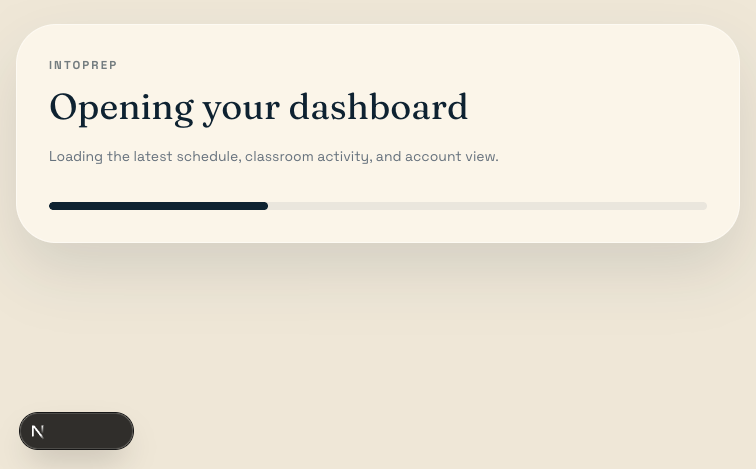
\includegraphics[width=\textwidth]{assets/staff-dashboard.png}

\subsection*{Staff Billing}
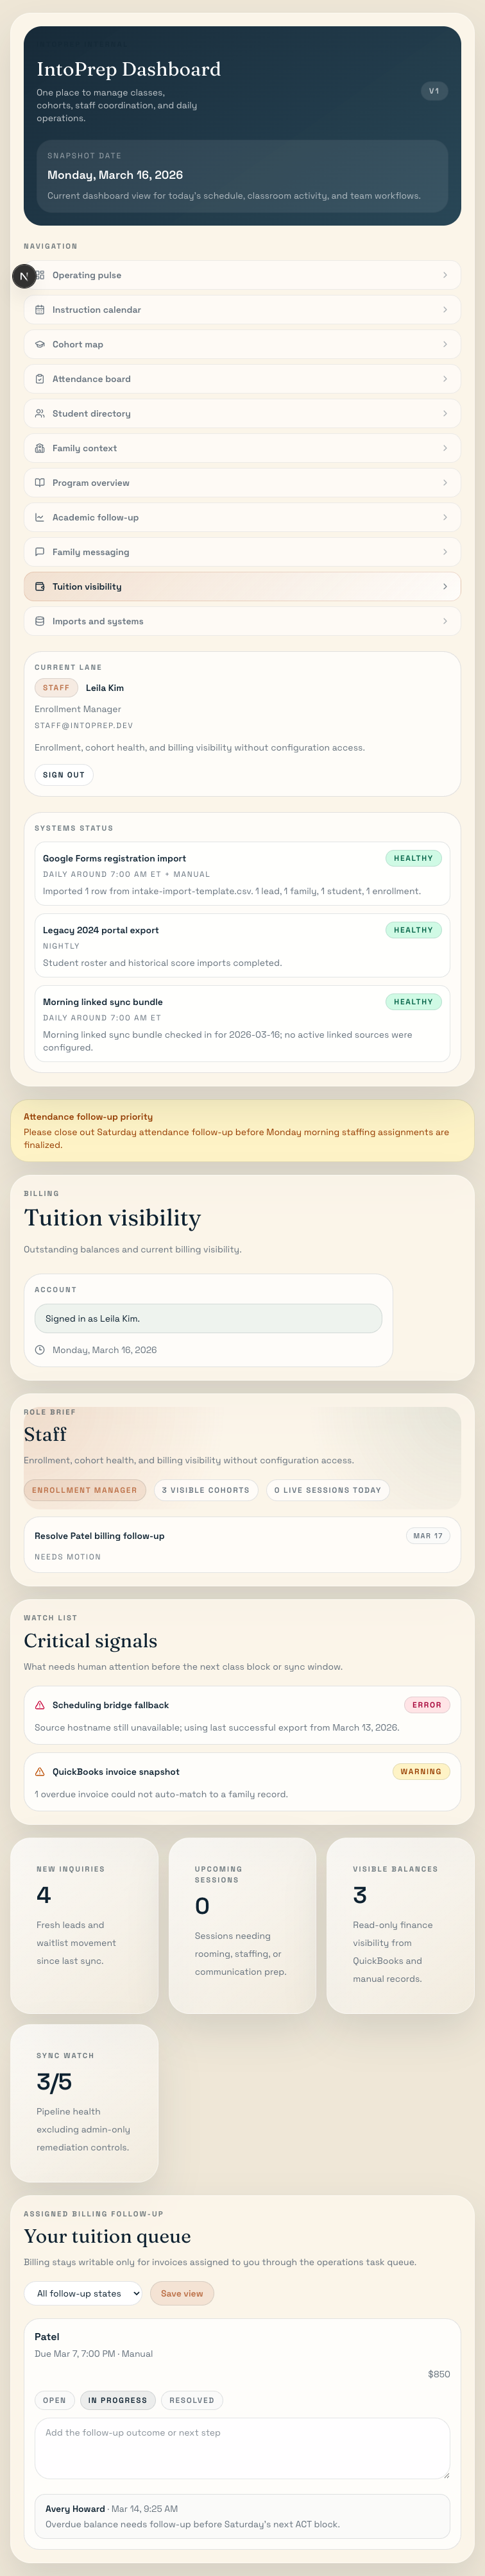
\includegraphics[width=\textwidth]{assets/staff-billing.png}

\subsection*{Staff Messaging}
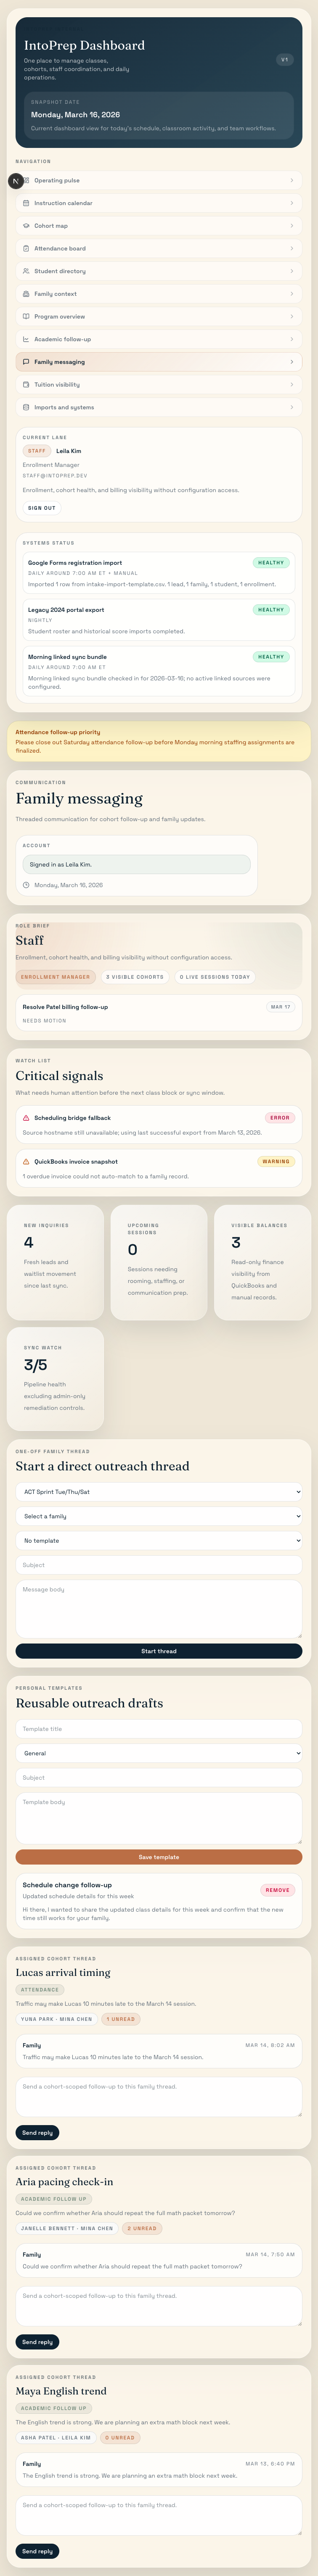
\includegraphics[width=\textwidth]{assets/staff-messaging.png}

\section*{First Login Walkthrough}
\begin{enumerate}
  \item Sign in at \texttt{/login}.
  \item Start on ``Operating pulse''.
  \item Review:
  \begin{itemize}
    \item assigned tasks
    \item overdue work
    \item claimed leads
    \item unanswered family communication
    \item assigned billing follow-up
  \end{itemize}
  \item Open ``Tuition visibility'' and confirm the billing lane is visible.
  \item Open ``Family messaging'' and review the current threads before replying.
\end{enumerate}

\section*{Daily Workflow}
\subsection*{1. Work Your Dashboard First}
Use the dashboard to decide what needs motion today.
\begin{itemize}
  \item overdue tasks
  \item overdue billing follow-up assigned to you
  \item blocked lead follow-up
  \item unanswered family threads
  \item sessions needing prep or closeout
\end{itemize}

\subsection*{2. Update Assigned Tasks}
When a task is assigned to you:
\begin{enumerate}
  \item Open the relevant work item
  \item Move the status as work progresses
  \item Leave a short progress, blocker, or handoff note
\end{enumerate}

Smoke test verification:
\begin{itemize}
  \item staff task update worked on the assigned billing follow-up task
\end{itemize}

\subsection*{3. Work Billing Only When It Is Yours}
Open ``Tuition visibility'' only for the items assigned to you.
\begin{itemize}
  \item review invoice context
  \item log follow-up progress
  \item keep the next handoff clear
\end{itemize}

Do not treat billing as a free-for-all queue. If it is not assigned to you, it should stay read-only.

\subsection*{4. Keep Family Communication Moving}
Open ``Family messaging'' to:
\begin{itemize}
  \item reply inside existing threads
  \item start new one-off threads when needed
  \item keep the message history current for the rest of the team
\end{itemize}

\subsection*{5. Use Integrations As A Watch Surface}
You can review sync health and run routine imports, but you should not expect to change source configuration or remediation state from the staff role.

\section*{Complete Capability Map}
Staff is the global execution role for day-to-day operations.

Use staff for:
\begin{itemize}
  \item assigned tasks and overdue queues
  \item lead ownership and follow-up
  \item session edits
  \item session prep and closeout tracking
  \item single-student cohort moves
  \item assigned billing follow-up
  \item family contact history and one-off messaging
  \item personal outreach templates
  \item approval requests and escalations
  \item personal saved views
  \item routine import monitoring and manual imports
\end{itemize}

Do not use staff for:
\begin{itemize}
  \item user governance
  \item billing exports
  \item cohort staffing changes
  \item archive and restore
  \item source configuration edits
\end{itemize}

\section*{How To Update A Task}
\begin{enumerate}
  \item Find the assigned task from the dashboard.
  \item Open the related workflow surface.
  \item Change the status:
  \begin{itemize}
    \item \texttt{open}
    \item \texttt{in\_progress}
    \item \texttt{done}
  \end{itemize}
  \item Add the note type that best matches the update:
  \begin{itemize}
    \item progress
    \item blocker
    \item handoff
  \end{itemize}
  \item Save the update so admins and TAs can see the latest context.
\end{enumerate}

\section*{How To Work A Billing Follow-Up}
\begin{enumerate}
  \item Open ``Tuition visibility''.
  \item Confirm the invoice or family is assigned to you.
  \item Review the last follow-up state and notes.
  \item Add the new action note.
  \item Move the follow-up state if needed.
  \item If blocked, escalate through the normal admin path instead of trying to bypass workflow.
\end{enumerate}

\section*{How To Claim And Work A Lead}
\begin{enumerate}
  \item Open the lead from the dashboard or intake-facing workflow.
  \item Claim the lead if it is unowned.
  \item Update stage, follow-up date, and notes as you work it.
  \item Release it only if ownership needs to move away from you.
  \item If another person should own it, ask admin to reassign it.
\end{enumerate}

\section*{How To Edit A Session Or Move One Student}
\begin{enumerate}
  \item Open the cohort or session view.
  \item Update only day-to-day session details such as title, time, room, or mode.
  \item For a student move, select one student and move only that enrollment.
  \item Read conflict warnings before saving.
  \item If the change affects staffing, cohort capacity, or multiple students, stop and use an approval request instead.
\end{enumerate}

\section*{How To Use Session Prep And Closeout}
\begin{enumerate}
  \item Open the relevant session workflow.
  \item Review the prep and closeout checklist state before the class begins and after it ends.
  \item Update the items that are complete so the rest of the team can see session readiness.
  \item Use notes or task updates if the checklist shows work is blocked.
\end{enumerate}

\section*{How To Use Family Contact History And Messaging}
\begin{enumerate}
  \item Open the family or thread.
  \item Read the existing history before adding a new note or message.
  \item Add the contact event with source and outcome when you complete a follow-up.
  \item Use a personal outreach template if it helps you stay consistent.
  \item Keep the message operational and specific to the current family need.
\end{enumerate}

\section*{How To Use Personal Templates}
\begin{enumerate}
  \item Create a template for common cases such as schedule change, missed attendance, score follow-up, or general outreach.
  \item Save it under your own account.
  \item Reuse it when starting a new one-off thread or replying inside a matching workflow.
  \item Update the wording as you learn what works, but keep it personal and not team-wide.
\end{enumerate}

\section*{How To Submit An Escalation Or Approval Request}
\begin{enumerate}
  \item Use escalation when work is blocked and admin attention is needed now.
  \item Use an approval request when you need permission for something outside your role, such as a bulk move or source change.
  \item Enter a clear reason and handoff context.
  \item Track the resulting status in your queue rather than assuming someone saw it elsewhere.
\end{enumerate}

\section*{How To Use Saved Views}
\begin{enumerate}
  \item Open the section you work repeatedly.
  \item Apply the filters you want to reuse.
  \item Save the view under a clear personal name.
  \item Reopen it from your saved-view list the next time you need the same queue.
\end{enumerate}

\section*{How To Use Integrations}
\begin{itemize}
  \item review sync health and recent import runs
  \item run a routine manual import when that is part of your workflow
  \item stop if the task requires source editing, remediation, or maintenance mode and hand it to admin or engineer
\end{itemize}

\section*{Guardrails}
\begin{itemize}
  \item no \texttt{settings} access
  \item no billing export
  \item no engineer incident tooling
  \item no archive or restore controls
  \item no reassignment of work owned by someone else
\end{itemize}

\section*{Verified Behavior}
Verified in the live browser pass:
\begin{itemize}
  \item staff login succeeded
  \item dashboard, billing, and messaging loaded
  \item staff task update succeeded through the real API
  \item direct access to \texttt{/settings} redirected back to \texttt{/dashboard}
\end{itemize}

\section*{Recommended First-Day Checklist}
\begin{itemize}
  \item review the dashboard queue
  \item open billing and confirm assignment-based follow-up
  \item reply to a real family thread only after reading the prior context
  \item update an assigned task so you understand the note types
  \item review the integrations page as a read-mostly health surface
\end{itemize}

\end{document}
\ No newline at end of file
